\title{Big Data in Safe Driver Prediction}

\author{Jiaan Wang}
\affiliation{%
  \institution{Indiana University Bloomington}
  \streetaddress{3209 E 10 St}
  \city{Bloomington} 
  \state{IN} 
  \postcode{47408}
}
\email{jervwang@indiana.edu}

\author{Dhawal Chaturvedi}
\affiliation{%
  \institution{Indiana University Bloomington}
  \streetaddress{2679 E 7th St}
  \city{Bloomington} 
  \state{Indiana} 
  \postcode{47408}
}
\email{dhchat@iu.edu}
    
\begin{abstract}

    For years, people have been trying to reduce their automobile
    insurance bills. Insurance companies claim that price will be
    reduced for good drivers and raised for bad ones. However,
    inaccuracies in their data predictions lead to the exact
    opposite. The data-set being used is released by Porto Seguro,
    an auto and homeowner insurance company from Brazil. It
    consists of information from several hundred thousands of
    policyholders. The goal is to predict the probability an auto
    insurance policyholder files a claim the next year using
    classification algorithms. A good prediction with decent
    accuracy can correctly adjust prices for policyholders.
    
\end{abstract}

\keywords{i523, HID233, HID204, Big data, Classification, Safe Driving, Predictive Analytics, Neural Networks}

\maketitle

\section{Introduction}

Everyday, people die from car accidents and it should come as no surprise that automobile accidents are one of the most common causes of death in the United States \cite{Suizo2015decisions}. As reported by the CDC, Centers for Disease Control, approximately over 40,000 people lose their lives to fatal automobile accidents each year. It should be clear that we need to enhance road safety for drivers all over the states \cite{Mills2017safety}. However, as we are currently in the age of big data, these automobile accidents could be prevented by using modern technologies and methods such as artificial intelligence and predictive analytics. 

Big data describes large quantities of data that are impossible to analyze using traditional data analysis methods. It includes structured and unstructured data. Structured data can be SQL database stores and unstructured data can be videos, images, social media feeds, etc. In industries, data analytics is often performed on big data in order to find specific patterns or anomalies that could prove useful for business decisions and choices. The amount of data is usually irrelevant in these cases. For example, smart cars utilize big data to improve their safety features and systems. They collect data such as driving patterns and routes as they travel from point A to B. This information is then sent to the computers on-board and gets transferred to the company servers where the data undergo analysis. The result is then collected and stored to enhance smart-car systems \cite{Walker2017safety}.

Big data is also helpful in providing insights for product development. It can find the causes for issues and problems in products through data analytics, which can then be used to improve the design. For example, the driver assistance feature on a Mercedes-Benz car not only has safety features but also collects data on driving habits. If large amount of drivers speed through intersections or break hard during traffic hours, the company can obtain these information and use them properly to enhance their systems for better road safety. They could add a detector with GPS data to spot intersections or traffic jams. Furthermore, another data that are useful to collect are driving routes. Google Street View utilizes big data from driving routes to update their maps and display views of different places \cite{Walker2017safety}.

Aside from smart cars, we also need to master data collection in order to know how automobile accidents happen. For example, the technology behind the famous black box, which tracks planes and cockpit communications to determine the reason behind crashes, is getting used in cars as well. It is not expensive nor complicated to apply this technology onto the majority of vehicles out there. By recording the precise time, locations, speed and other variables, this technology can definitely help us collect valuable data and information in car accidents. The result from data analysis can also assist us in a deep understanding of causes behind automobile collisions in order to save more lives by preventing future accidents. The first country who thought to implement this technology on cars was South Korea. As a result, in the following year, a 14 percent decrease was saw in the number of car accidents along with a 20 percent decrease in the number of injuries and deaths of fatal automobile accidents \cite{Mills2017safety}.

Predictive analytics is a powerful method in big data analytics to help predict future events or outcomes based on current and historical data. It usually utilizes big data techniques such as data mining, predictive modeling and statistics. It uses a wide range of predictive models which depends on the type of event we are predicting. For example, most predictive models produce a number called a score where a higher score indicates a higher chance of that outcome happening in the future. It is a very useful tool for making business decisions and assessing potential risks in many industries such as insurance, retail, etc. Predictive analytics does not inform users about things that has happened before today. It tries to predict for a particular driver the probability that he or she may be involved in an car accident in the near future or any other chose time as accurately as possible \cite{Suizo2015decisions}.

For example, in order to find high-risk drivers, it is not enough to just have driving records, automobile incident reports or traffic tickets. We also need something called telematics. Telematics is defined as the combination of telecommunications and informatics. It collects, stores, sends and receives data and information via transmission-enabled devices. For example, the use of the car black box technology mentioned previously to collect and obtain information on driving behaviors or patterns is called vehicle telematics. With telematics data, companies can determine the possibility of a driver in a future car accident along with the expenses coupled with it. They can also take actions such as putting high-risk drivers into training schools to correct their bad driving behaviors before an incident happens \cite{Suizo2015decisions}.

By studying the telematics data from a specific driver, we can learn his or her driving behaviors and create a report that details the potential danger this driver may inflict and use these data to correct those bad driving habits. The probability of a driver being involved in a car accident in the future can be used to categorize drivers into different groups. With these probabilities, companies can create a safety score to provide them with suggestions on which drivers to deal with first. The fundamental role for a safety score is to identify drivers with high risks before an accident happen to give the driver a chance to correct those bad driving habits and prevent incidents from happening \cite{Suizo2015decisions}.

However, just like other countless programs on risk evaluation, predictive analytics is not supposed to be flawless. In companies such as UPS, FedEx, USPS or any other services that use a large amount of drivers and vehicles called fleet vehicles, predictive analytics is just the first process and it requires the total cooperation and commitment from the company, drivers and fleet staff to achieve the highest efficiency. Companies that have numerous successful fleet operations are those who plan ahead and bring together all fleet personnel into the action. The most effective way to adjust the accuracy and preciseness of predictive models is to test the models every few days or few weeks or any other time that is suitable for the operations. Due to the fact that most operations have tight schedules, this leeway time will give companies enough room to call in safety personnel to step in to either train drivers to correct their driving habits or repair fleet vehicles beforehand to avoid major system failures \cite{Suizo2015decisions}.

Predictive analytics and telematics data are being used in almost all fleet companies as more of them start to see the value in predictive analytics. With the help of predictive analytics, fleet companies can be actively engaged in making better decisions about their fleets and companies by improving road safety, reducing expenses and risks or decreasing work load time \cite{Suizo2015decisions}.

\section{Big data in the insurance industry}

For a long time, auto insurance companies have calculated insurance rates based on personal mileage through out the years \cite{Fung2016turn}. Traditional auto insurance companies categorize users by demographics such as gender and other factors such as education. They then make predictions based on past statistics about their chances of getting involved in future car accidents. This means that the monthly payments insurance companies charge you are only calculated according to the information they have on you and these information has nothing to do with your driving behaviours. As a result, the premiums you pay every month is usually based on past data from people who have identical demographics as you. While a few of the factors are actually helpful in determining your risk score - for example, if you have had multiple accidents in the past, you are likely to be involved in a new one in the future - other factors such as how many cars you previously owned have little to do with your actual risk of being in an accident but yet they still matter when calculating the price. And no one ever use the most important factor in determining monthly premiums which is driving behaviors \cite{Rippe2017unfair}.

Major auto insurance companies have connection to large amount of information as well as data processing power in order to calculate risk scores and monthly premiums. It is no easy task for them to combine several different factors into one single price. Still, big data is not fully utilized. Even though these companies use a variety of different models to calculate monthly rates for drivers, not all of their methods are optimized. In a study conducted earlier this year, it was found, with the help of data mining, that there exists predictive models that have higher accuracy in categorizing drivers into high and low risk groups. Among those models was one that combined 16 factors which produced an extremely high accuracy in risk assessment \cite{Rippe2017unfair}.

Big data can help insurance companies in a big way to make better and smarter business decisions. 

\begin{itemize} 

    \item Financial fraud has always been a big problem for both insurance companies and their clients ever since the invention of insurance. The expense that insurance fraud inflicts each year is more than 40 billion dollars as reported by the FBI. However, insurance companies now can put big data into good use as a brand new approach in detecting insurance fraud. Coupled with immense computing power and complex mathematical algorithms, insurance companies are now able to analyze their data to find abnormalities which might indicate possible fraud. For example, a variety of applications and computer software now have the ability to detect outliers automatically in the data. However, the anomalies detected do not always turned out to be fraud situations. There could be other reasons or explanations for them but this new approach certainly makes insurance companies a lot easier to detect potential fraud \cite{Cordray2015data}.
    
    \item Another benefits for insurance companies to use big data is that big data analytics applications such as Apache Hadoop are engineered to be simple to use with office software such as Excel. As a result, it is much easier to write reports in Hadoop which is intended to work with Excel. Insurance staff can now access huge amounts of data swiftly to obtain the information they need and produce a report in the form they already know how to use \cite{Cordray2015data}.
    
    \item Two years ago Google released a tool for residents of California to compare rates among different auto insurance companies. Since then, the competition has been increasing in the industry. However, there is no need for this useless competition because big data can help insurance companies find better ways to provide their customers with a good price while still earning profits. By collecting data and customer information from various sources such as social media, insurance companies can utilize these big data to accurately predict which customers are likely to file claims in the future and then try to bring in more of these customers \cite{Cordray2015data}. 
    
    \item Aside from auto insurance, big data also has some interesting applications in the industry of health-care. With the accurate and effective collection of data on medical records, insurance companies can provide better health insurance plans for people so that they can have longer and better lives. As a result, people with better health insurance plans file less claims which means insurance companies spend less money and earn higher profits. For example, insurance companies can advertise wearable technologies or devices such as apple watch to track customers well-beings in order to provide them with incentives to exercise or obtain better lifestyles \cite{Cordray2015data}. 
    
    \item The insurance industry is continually changing. Insurance companies that can not match the pace will lose profits and resources. However, using big data, insurance companies can study and learn real time data such as social media feeds to obtain more information about customer styles and preferences. This can help insurance companies to design better marketing strategies, adapt faster to customer feedback and construct products that are more attuned with their customers' tastes \cite{Cordray2015data}.
    
    \item Last but not least, big data can also help insurance companies to provide insurance plans that are tailored to their customers. Every year, millions of money is lost because insurance companies do not have the means to personalize their insurance plans. However, with the help of big data analytics tools, employees in insurance companies now have the ability to gather more precision information on every one of their customers with ease so that they could create insurance plans according to each individual's needs. These tools and software can also give insights and advice based on the collected data to provide better support for employees to make decisions. This in turn will increase their customer satisfaction and lead to more customers in the future \cite{Cordray2015data}.

\end{itemize}

However, powered with advanced technology and big data analytics, insurance companies now-days have access to customers' driving behaviours for more personalized insurance rates. They collect specific data on how often you drive every day, how long you drive each time, how often you speed, how often you break hard and so on to determine the probability of you being in an accident in the near future. With these precise data on each individual customer, insurance companies can assess risk scores for everyone and use that information to calculate your monthly rates \cite{Fung2016turn}. For example, an auto insurance company called Root is one of the first mobile auto insurance companies that are intended to help you on the go. They promise to only insure the good drivers to make sure they get the best rates. Their methods are simple. Download the app, take a test drive with the app on-board for several weeks and Root will send a personalized premium plan based on your driving behavior. Then you can just select the plan you want to purchase and buy via your phone \cite{Rippe2017unfair}.

These new and innovative mobile auto insurance plans are called UBI, short for Usage-Based Insurance and they calculate monthly premiums mostly based on driving habits. Applications on smart-phones and on-board diagnostic devices along with in-car tracking technology from manufacturer are used to record mileage and driving behaviours. 
These mobile insurance programs tend to give discounts for good drivers as a reward for their good driving behaviors. They are even adding new rewards such as roadside assistance on top of discounts for drivers who have maintained good driving behaviors for long periods of time. By collecting big data on driving habits, auto insurance companies can promptly discover mistakes when accidents happen by knowing the exact positions of each car and driving habits data such as speeding or braking as well as environmental data such as weather or road conditions \cite{Shafer2016industry}.

On the surface, these Usage-Based Insurance plans appear to be plausible and feasible. An application or a sensor is installed on your phone or car to track your driving behavior instead of estimating costs based on factors such as age, gender, education, traffic records, accident reports and so on. Several programs such as {\em Drivewise} from Allstate insurance and {\em Snapshot} from Progressive insurance have been released to the public for a couple of years in some states, completely based on customers' choices. You do not have to install them if you do not want to. However, the majority of drivers have been embracing these monitoring devices since it has no apparent downside. As long as your driving behaviors are considered to be safe, such as slow braking and accelerating or no driving around midnight, your should receive discounts like 5 to 10 percent or even up to 20 percent on your monthly premiums. On the other hand, customers are starting to worry about their privacy but we still do not know what the worst thing that might happen if we keep letting insurance companies monitor our driving behavior. According to the Wall Street Journal, these Usage-Based Insurance plans are growing exponentially. The biggest auto insurance company in United States, State Farm, announced their plans to expand their {\em Drive Safe and Save} program to the entire country soon. Their major advertising strategy is that by enrolling in the program, consumers can get discounts in their insurance premium by proving that they drive safely \cite{Tuttle2013habits}.

For example, one of the earliest Usage-Based Insurance programs available to the public was released about 10 years ago by Progressive and General Motors. This particular program, with the help of GPS, applied discounts based on customer mileage. Many of the Usage-Based Insurance programs these days still implement this strategy but many improvements have been made. Insurance companies nowadays know everything about the way you drive from where you drive to when you drive as well as how you drive. There are also a variety of options to choose from such as {\em pay as you drive} and {\em pay how you drive}, thanks to telematics. The advantage of having telematics in these insurance programs is to improve efficiency such as reducing response time for accidents. In addition, Usage-Based Insurance data can be analyzed using on-board diagnostic devices which are often plugged in via the on-board diagnostic 2 port on cars. These diagnostic devices do not have the ability to track car positions but they do generate more precise and meticulous data about car usage. Although telematics is the typical way to record driving habits, new creations in the future will possibly use smart-phone's location services or GPS abilities to track bad driving behaviors such as speeding and hard braking. Liberty Mutual and State Farm both tested their new tracking technology via smart-phones or other smart devices on-board cars in 2015. By 2020, the majority of auto insurance companies will be using Usage-based Insurance programs coupled with telematics data. It is no doubt that Usage-Based Insurance programs will continue to grow and achieve even higher precision and availability \cite{Firm2016insurance}.

\section{Current Applications}

Predictive analytics are being utilized with telematics data to enhance and improve road safety. Telematics have been used for a long time in insurance industry to monitor driving behaviors such as speeding to identify high-risk drivers. Now coupled with predictive analytics, these data are being analyzed to predict the likelihood of a driver being involved in future accidents. SmartDrive Systems, a transportation safety and intelligence company, employs even more interesting ways to predict accidents. They record and gather video feeds from dashboard cameras in cars which are then integrated with telematics data. This way, they can improve their predictive analytics on driver safety and eventually leads to better predictions \cite{Banker2016accident}.

SmartDrive Systems uses a private cloud to provide their clients with predictive analytics solutions. All the data from their clients are collected by the company and stored on their cloud. The data includes telematics and video feeds from millions of clients with more than 4 billion mileage. SmartDrive constantly improves their predictive models because the agreements SmartDrive has with their clients permit them to study all the data they gather. The usage of both telematics data and video feeds is a great idea which enables SmartDrive researchers to better understand the data and interpret the results. By combining what they see through the video feeds and the results from telematics data analysis, the researchers can draw conclusions such as making a U-turn on a narrow road within some fixed radius is dangerous \cite{Banker2016accident}.

Indiana State Police came up with a different way to predict incidents and are making their predictive analytics methods open source. In their approach, they produced something called {\em Daily Crash Prediction Map} which finally completed in November. It contained data such as accident reports from all the police departments in Indiana going back to 2004 as well as data on daily weather, historical traffic amount and so on. This map highlights where potential accidents may happen categorized by their probabilities. It also features information about past accidents such as locations, dates, causes, fatalities and so on \cite{Bergal2017sites}.

Liberty Mutual is the nation's third largest property and casualty insurance company. Last year, Liberty Mutual partnered up with Subaru. In doing so, customers was granted access to {\em Starlink}, Subaru's multimedia and navigation system, which can track and notify drivers via an app if they are speeding or braking too hard. By enrolling in the {\em RightTrack} program provided by Liberty Mutual, drivers can get up to 30 percent discounts for good driving behaviors \cite{Fung2016turn}. 

\section{Data Analysis}
The data we are gonna use for our analysis is of Porto Seguro. It is one of Brazil's largest auto and homeowner insurance companies. Inaccuracies in car insurance company's claim predictions raise the cost of insurance for good drivers and reduce the price for bad ones. The task is to build a model that predicts the probability that a driver will initiate an auto insurance claim in the next year or not. An accurate prediction will allow them to further tailor their prices, and hopefully make auto insurance coverage more accessible to more drivers. 

\subsection{Approach}
We will be mainly discussing about the Exploratory data Analysis we have  performed on the data until now. We will be using the help of both R and python environment and supporting packages to perform the necessary statistical analysis. Along with this, we will discuss  about  the  Machine  or  Deep  Learning  algorithms  / models that we will be using to achieve the near solution for the problem.

\subsection{Feature Information}

Dimensions of the data [Rows x Features] : [ 595212, 59 ]
 
The data-set constitutes different varieties of features.
 
 \textbf{Binomial Features} [Count : 17] :  ps\_ind\_06\_bin,  ps\_ind\_07\_bin, ps\_ind\_08\_bin, ps\_ind\_09\_bin, ps\_ind\_10\_bin, ps\_ind\_11\_bin, ps\_ind\_12\_bin, ps\_ind\_13\_bin, ps\_ind\_16\_bin, ps\_ind\_17\_bin, ps\_ind\_18\_bin, ps\_calc\_15\_bin, ps\_calc\_16\_bin, ps\_calc\_17\_bin, ps\_calc\_18\_bin, ps\_calc\_19\_bin, ps\_calc\_20\_bin.

 \textbf{Categorical Features} [Count : 14] : ps\_ind\_02\_cat,  ps\_ind\_04\_ cat, ps\_ind\_05\_cat, ps\_ind\_01\_cat, ps\_ind\_02\_cat,  ps\_ind\_03\_cat, ps\_ind\_04\_cat, ps\_ind\_05\_cat, ps\_ind\_07\_cat,  ps\_ind\_06\_cat, ps\_ind\_08\_cat, ps\_ind\_09\_cat, ps\_ind\_10\_cat,  ps\_ind\_11\_cat.

 \textbf{Integer Features} [Count : 16] : ps\_ind\_01, ps\_ind\_03, ps\_ind\_14, ps\_ind\_15, ps\_ind\_11, ps\_calc\_04, ps\_calc\_05, ps\_calc\_06, ps\_calc\_07, ps\_calc\_08, ps\_calc\_09, ps\_calc\_10, ps\_calc\_11, ps\_calc\_12, ps\_calc\_13, ps\_calc\_14.

 \textbf{Floating Features} [Count :10] : ps\_reg\_01, ps\_reg\_02, ps\_reg\_03, ps\_calc\_01, ps\_calc\_02, ps\_calc\_03, ps\_car\_12, ps\_car\_13, ps\_car\_14, ps\_car\_15.
 
The remaining two features constitutes \textbf{id} and the \textbf{output (or) target}. 
All the features has been clearly represented using post script, \textbf{\_cat} for categorical data, \textbf{\_bin} for binomial data.
 
The \textbf{missing values} in the features are represented by -1.

\subsection{Data Pre-processing}

As shown in \ref{f:missing}, missing values are found in 14 of the 58 columns. There are 6 features with more than 5000 missing row values. Owing to the shear size of the unavailable data, we have not performed any missing value treatment and removed these features from consideration. Of the remaining data, across rows, data is unavailable in almost 500 ($<$1\%) rows and these are promptly removed.

\begin{figure*}
  \centering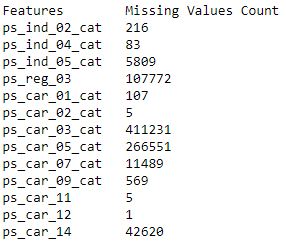
\includegraphics[width=\columnwidth]{images/missingdata}
  \caption{Missing Data}\label{f:missing}
\end{figure*}

\subsection{Distribution of the target variable}
As shown in \ref{f:numerical}, target variable claims is a binary variable with a skewed distribution of classes. 96\% of the customers didn't make any claims. We wish to consider this distribution in measuring classification accuracy. Area under the ROC curve, recall and precision would be relevant metrics in this case.
 
\begin{figure*}
 \centering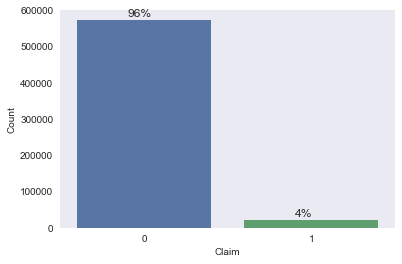
\includegraphics[width=\columnwidth]{images/target}
 \caption{Target Variable Distribution}\label{f:numerical}
\end{figure*}

\subsection{Numerical Predictors (vs) Target Variable}

 Average value of most of the numerical predictors is higher when the claims are filed. This is a unique phenomenon and we intend to use this contrast in predicting the target variable.
  
\subsection{Artificial Neural Networks}

Artificial neural networks (ANNs)  are computing models which are based on biological neural networks that constitute human brains. The idea of ANNs is based on the belief that working of human brain can be imitated for computers by using silicon and wires as living neurons. Such systems learn by progressively improving their performance to do tasks by considering examples, generally without task-specific programming. ``The human brain can be considered as a complex network of nerve cells called neurons(about 86 billion)'' \cite{Ainet}. They are inter-connected to other millions of cells by Axons. These neurons then react to stimulation from external environment or inputs from other organs. A neuron can then send the message to other neuron to handle the issue or does not send it forward. 

ANNs also try to imitate biological neurons of human brain. The neurons are connected by links and they interact with each other. The nodes can take input data and perform simple operations on the data. The result of these operations is passed to other neurons. The output at each node is called its activation. Each node is assigned with weight. ANNs are capable of learning, which takes place by altering weight values. If the network generates the desired output, there is no need to adjust the weights. However, if the network generates an undesired output or an error, then the system alters the weights in order to improve subsequent results.

\subsection{Types of ANNs}

\subsubsection{Feedback ANN}

In this type of architecture, the output goes back into the network to achieve the best-evolved results internally. The feedback network feeds information back into itself and is well suited to solve optimization problems. Feedback ANNs are used by the Internal system error corrections \cite{Neuralnet}. 

\subsubsection{Feed Forward ANN}

A feed-forward network is a neural network which consists of an input layer, an output layer and one or more hidden layers of neurons. By evaluating its output by changing its input, the efficiency of the network can be noticed based on group behavior of the connected neurons and the output is decided. The main advantage of this network is that it learns to evaluate and recognize input patterns  \cite{Neuralnet}.

\subsubsection{Radial Basis Function Neural Network}

The RBF neural network is the first choice when interpolating in a multidimensional space. The RBF neural network is a highly intuitive neural network. Each neuron in the RBF neural network stores an example from the training set as a ``prototype''. Linearity involved in the functioning of this neural network offers RBF the advantage of not suffering from local minima \cite{Neuralnet}.

\subsubsection{Kohonen Self-Organizing Neural Network}

``Invented by Teuvo Kohonen, the self-organizing neural network is ideal for the visualization of low-dimensional views of high-dimensional data. The self-organizing neural network is different from other neural networks and applies competitive learning to a set of input data, as opposed to error-correction learning applied by other neural networks. The Kohonen self-organizing neural network is known for performing functions on unlabeled data to describe hidden structures in it'' \cite{Neuralnet}.

\subsubsection{Recurrent Neural Network}

The recurrent neural network is a neural network that allows a bi-directional flow of data. The network between the connected units forms a directed cycle. Such a network allows for dynamic temporal behavior to be exhibited. The recurrent neural network is capable of using its internal memory to process arbitrary sequence of inputs. This neural network is a popular choice for tasks such as handwriting and speech recognition \cite{Neuralnet}.

\subsubsection{Classification-Prediction ANN}

It is a subset of feed-forward ANN and the classification-prediction ANN is applied to data-mining scenarios. The network is trained to identify particular patterns and classify them into specific groups and then further classify them into patterns which are unique for that network \cite{Neuralnet}.

\subsubsection{Physical Neural Network}

This neural network aims to emphasize the reliance on physical hardware as opposed to software alone when simulating a neural network. An electrically adjustable resistance material is used for emulating the function of a neural synapse. While the physical hardware emulates the neurons, the software emulates the neural network \cite{Neuralnet}.

\subsection{Data Analysis Using Neural Networks}

Rather than beginning our inquiry into the data-set with more traditional methods like regression we straight away tried to learn Artificial Neural Networks. Logistic regression itself, can be thought of as a special case of a neural network with a single neuron (~perceptron). 

After studying and learning the theory behind ANNs we proceeded to learn how to implement them -- by ourselves at first, and later using TensorFlow. So far we have tried quite a bit of different models and learned some lessons about the data.

\begin{itemize}

\item \textbf{Data Cleaning :} As pointed out by the EDA above, there were a few columns which had a lot of missing data. For columns which had $>1000$ values missing (~6 columns), we disregarded them altogether. For the remaining data points, we disregarded the rows which had any one particular value missing. We started with a simple data cleaning strategy so as to not complicate it too much at the initial stages, but we will probably want to look at it again as we go along.

\item The first thing that we tried is using a simple \textbf{perceptron}. The input layer had 51 nodes (after removing the id, target and 6 other columns in data cleaning) and the output layer had a single perceptron with a sigmoid activation function. The best score that we got when we uploaded our code to Kaggle was $0.03$ whereas the leader-board is hovering around $0.290$ so this is not too impressive.

\item However, now we added more hidden layers and nodes to see if we get a better job of fitting the data. To start off, we only consider the continuous variables so that we don't have to worry about handling binary/categorical data. We have $24$ nodes in the input layer. The final layer has one node  since it is a classification problem. We kept all activation to be logistic and experimented a bit with the number of hidden layers and nodes to get a best score of \textbf{0.211} with this simple approach.

\item \textbf{Issued Encountered}  Looking at the results from the neural network there is one major issue. Whenever we add too many hidden layers ($>3$) the outputs for the test data are all $\approx 0$ and the score drops. After some trial and error, we have diagnosed the issue to be the biased nature of the training data (~$96\%$ of the training data are $0's$). So the ANN sees too many zeros and consequently predicts mostly zeros. We aim to explore different sampling methods to train the neural network to improve the results further (along with cross validation which we haven't implemented).
\end{itemize}

\section{Other Techniques that can be used}

Among the machine Learning algorithms that are used in practice, gradient tree boosting is one technique that shines in many applications.Tree Boosting has been shown to give many state of the art results for many standard classification problem.

The most important factor for the success of XGBoost is its ability to scale in all the scenarios. The XGBoost algorithm run ten times faster than the existing popular solutions on a single solution and scales to billions of example in distributed or memory-limited settings.

The Porto Seguro data-set is clearly an classification problem, the data will be having only two outputs either the car insurance holder is going to claim or not.

While domain dependent analysis and feature engineering plays an important role in defining or modeling the solutions, the fact that XG Boost is the consensus choice for learners shows the impact and importance  of our system in tree boosting.One problem with the Porto Seguro data-set we do not have have much information about the Features and all the feature must have to under go through strict statistical treatment to build an optimal solution.

\section{Conclusion}

Reducing insurance rates has always been a difficult task in the past. However, armed with advanced technology, insurance companies now have the ability to track personal driving behaviours to provide better suited personalized insurance plans. We performed Neural Networks algorithm on clients data from Porto Seguro, one of Brazil's largest auto insurance companies in order to predict the probability of drivers filing claims in the next year. Our analysis proved to be a success and our model yielded a high accuracy.


\section{Appendix}

\subsection{Links to iPython notebook:}

\url{https://github.com/bigdata-i523/hid233/blob/master/project/Shallow_Neural_Nets.ipynb}

\subsection{Links to iPython notebook pdf version:}
\url{https://github.com/bigdata-i523/hid233/blob/master/project/Shallow_Neural_Nets.pdf}

\subsection{Work Contribution}

Jiaan Wang - Sections: Abstract, Introduction, Big data in the insurance industry, Current application, Data analysis (10 percent) and Conclusion

Dhawal Chaturvedi - Sections: Data analysis (90 percent), Other techniques that can be used and Conclusion as well as Jupyter notebook


\begin{acks}

  The authors would like to thank Dr. Gregor von Laszewski for his
  support and suggestions to write this paper.

\end{acks}

\bibliographystyle{ACM-Reference-Format}
\bibliography{report} 

